\documentclass{IEEE}

\begin{document}
\Title{Machine Learning From Disaster}{Calculating the Survival Rate for Passengers in the Titanic}
{Miguel Melo Ochoa}{Alex Hayet}{Francisco Gomez}{Maeki Kashana}
{CS549 - Machine Learning}
{Professor Xin Zhang}
{San Diego State University}


\section{Introduction and Research Problem}
All details for this project will be provided by a competition titled "Titanic - Machine Learning from Disaster" introduced by kaggle.com \cite{titanic}.

This following section will provide a brief background and a statement of the problem this project is addressing.




\subsection{Introduction}

This project will build a predictive model that aims to find the type of people who are going to survive the sinking of the Titanic, a well renowned ship that was believed to be "unsinkable" until it hit an iceberg in 1912, resulting in the death of 1502 passengers/crew.

This project will utilize passenger information, such as name, age, gender, socio-economic class, etc., to determine what sorts of groups were more likely to survive than others during the sinking of the Titanic.

This data aforementioned above will be provided by the Kaggle competition and the goal of this project is to engineer code that uses the data to calculate the survival rate of various groups of people.

\subsection{Research Problem}

This project will be creating a predictive model that will dictate the type of individuals that were the most likely to survive the sinking of the Titanic.

To give more detail, this project will be provided with a lot of testing data in order to make predictions on who will survive. In consequence of this data, this team will be able to create a predictive machine learning model that utilizes the data provided for this project to make predictions using various models previously covered in this course. The specific details regarding any related work that relates to this project will be discussed in depth in later sections.

To get more into specifics, this project will utilize these following .csv files to find a solution for this problem: test.csv and train.csv.


For the train.csv file, it will contain information on who survived the sinking of the Titanic in order to train the model that was developed.

For the test.csv file, it is used to see how well the model that was developed performs on unseen data. This file will be used to make predictions on who survived based on the model that was trained using train.csv.




\section{Related Work}

To create a solution for this project, our code needed to apply the concepts that were learned about logistic regression. To aid with this endeavor, our team utlized the problems that involved logistic regression in Assignment 1.

In this assignment, there was a task that involved training a logistic regression model that classifies two categories of sign language images. Furthermore, through this assignment, we used the forward and backward computation implementation as a reference on implementing a logistic regression model in our own code.

More specifically, our team utilized the equations present in these computations in Assignment 1 and applied them in our code to produce a solution to the Titanic problem. In the forward pass, our team utilized these equations for the activation and the cost: $A=\sigma (w^TX+b)$ and $Cost=-\frac{1}{m}\sum^m_i y^{(i)}log(a^{(i)})+(1-y^{(i)})log(1-a^{(i)})$. In addition, for the backward pass computations, our team utilized these following equations from Assignment 1:
\LIST{
\item $dZ=A-Y$
\item $dw=\frac{1}{m}XdZ^T$
\item $db=\frac{1}{m}np.sum(dZ)$
}
These equations were used to compute the gradients $dw \text{ and } db$ as well as the cost. Afterwards, our code then utilized these gradients and returned them in the code, much like the code in Assignment 1.

Furthermore, another necessary part of our code was the sigmoid function, which we used to implement our logistic regression model. What our team used to implement the sigmoid function was the example of a sigmoid function shown in Assignment 1.

In this part of the assignment, my team utilized the equation for the sigmoid function, which was $\sigma(z) = \frac{1}{1+e^{-z}}$, in order to implement our own sigmoid function to solve our Titanic problem. Additionally, our team also used the code present for the sigmoid function in Assignment 1 as a reference when implementing our own version of the sigmoid function.

In addition to the sigmoid function, our team also needed to create/implement a function for the gradient descent. In our code, the gradient descent function was vital to our logistic regression model and we had used the example of a gradient descent function present in Assignment 1. In the assignment, it shows that the gradient descent function calls another function, which was $forward_backward()$ that run for $num_iters$ times. We used the same methodology in the gradient descent function present in Assignment 1 when we implemented our own gradient descent function for the logistic regression model.

Furthermore, in the gradient descent function shown in Assignment 1, it was described that the parameters that were passed in, $w$ and $b$, are updated within each iteration of the gradient descent algorithm. The equation for how to update these parameters were given in Assignment 1 and our team used the same equations to update the parameters in our own gradient descent function. These equations for these parameters were as follows:
\LIST{
\item $w=w-\alpha$
\item $b=b-\alpha \cdot db$
}
Lastly, our team implemented the function to make predictions. Like always, our team used the "predict" algorithm in Assignment 1 as a reference for the making of our own prediction algorithm. Using the example in Assignment 1, our team was able to compute the activation and convert probabilities to real predictions. This example in Assignment 1 allowed our team to effectively a prediction algorithm to predict who will survive and who will persih in the sinking of the Titanic.

Finally, our team's last task was to integrate all of the functions that we have created in the code thanks to the examples shown in Assignment 1 into one single model. To do this, our team, once again, used the model present in Assignment 1 as an example. Using the example model, our team was able to create one singular model that integrates all the functions that were discussed previously and applied the model on our own train data and then evaluated on the test data. In addition, our team also calculated the evaluation metrics for our own code to solve the Titanic problem, which used the example present in Assignmnet 1 to do so.
\section{Methodology and Technical Details}

\subsection{Methodology}
    What our team for the Titanic problem ended up doing was utilizing the logistic regression model as shown in Assignment 1 of this course. This is due to the scenario providing a set of given independent variables, involving classifications, and having to predict one of only two possible outcomes. The logistic regression model is optimized in finding patterns in multiple variables like these to make accurate predictions as to whether the outcome will be one thing or the other. Half of the columns provided in the Titanic passenger data happen to have correlations between a passenger having a certain value and that passenger surviving. In order to even begin, we would have to consider which of those columns would actually increase our accuracy and then eliminate the ones that are no help. Something else to consider is that some of the data is either missing or comes in a type that isn’t as easy to use. To address that, we will have to carefully fill up the empty slots with reasonable values and replace others with better types. Logistic regression makes use of the sigmoid function, processes like forward and backward propagation, and algorithms such as the gradient descent.
\subsection{Technical Details}
In regards to the technical details of our code, the two possible outcomes are the person surviving or perishing which are represented as 1 and 0. The independent variables we ended up utilizing were Pclass, Sex, Age, SibSp, Parch, and Embarked. Some of these variables, such as sex, are given as strings so they were changed to binary to make it more convenient to use. This is determined by whether the given passenger’s Sex is male or female and whether their Embarked is Q or S. A few areas also contain nan or “not a number” that had to be replaced with the average value of that category to maintain the patterns found and avoid errors. Once those columns of the Titanic’s passenger data are filtered and modified, it is used to train the model to recognize certain patterns on what increases someone’s chances of survival. That will allow it to make accurate predictions on whether a passenger will survive.

\section{Experimental Results and Analysis}

\subsection{Experimental Results}
Our experimental results for this project are shown in the graphs below. These graphs depict the survivors of the titanic according to our logistic regression model and also these graphs show how the accuracy of the model continues to drop the more iterations there are in the algorithm.

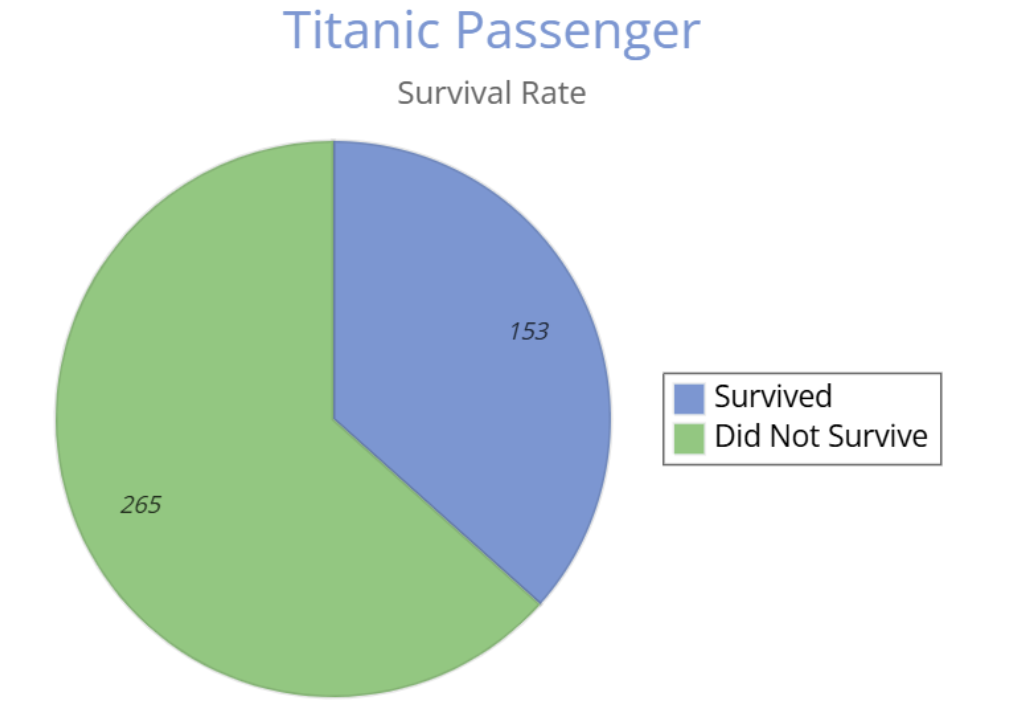
\includegraphics[scale=0.535]{./piechart.png}
\\ 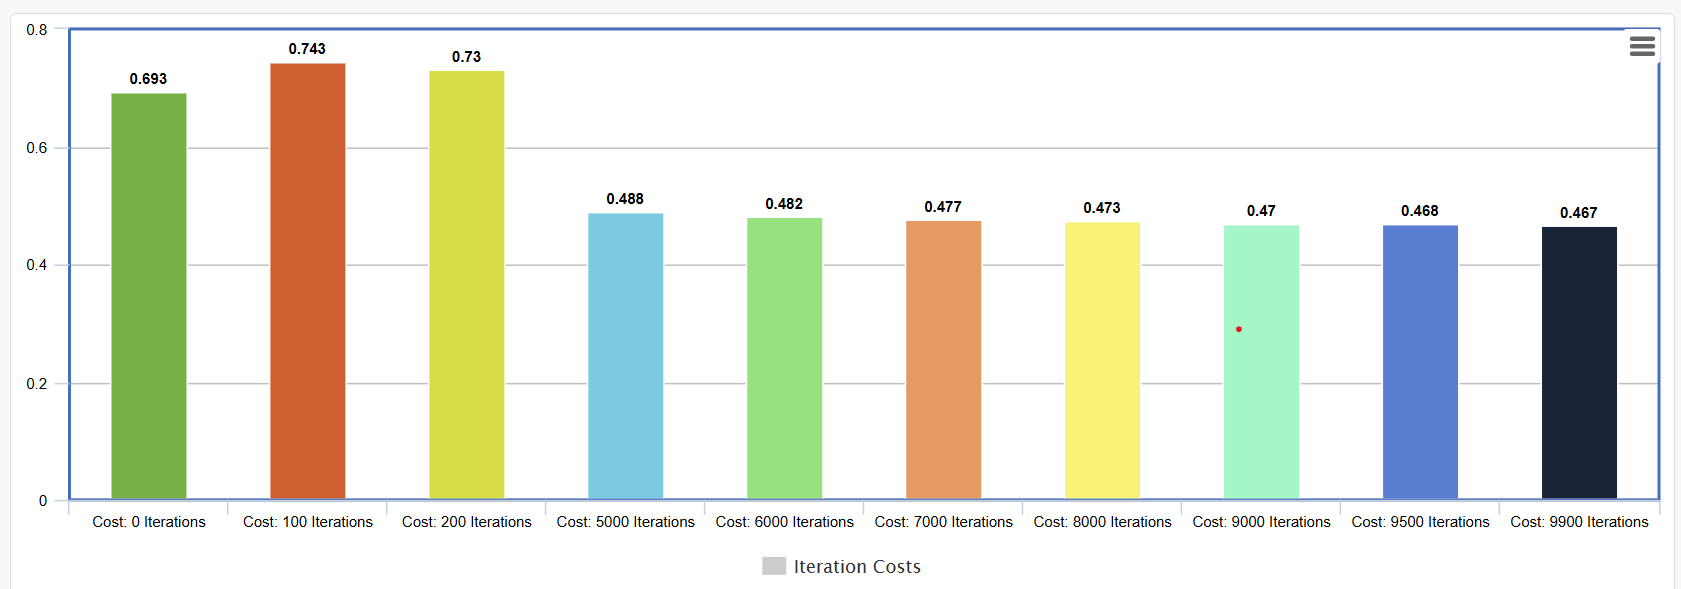
\includegraphics[scale=0.32]{./barchart.png}

Looking at the results of the titanic experiment, the results are defined using binary classification. This means that all results will be either 0 or 1. A 0 means that the passenger did not survive the titanic sinking while a 1 indicates that the passenger did in fact survive. In the experiment there were a total of 418 passengers aboard the titanic. Out of the 418 passengers, 153 survived and 265 did not survive the tragedy. This leaves us with a 36.6\% survival rate among all of the passengers.
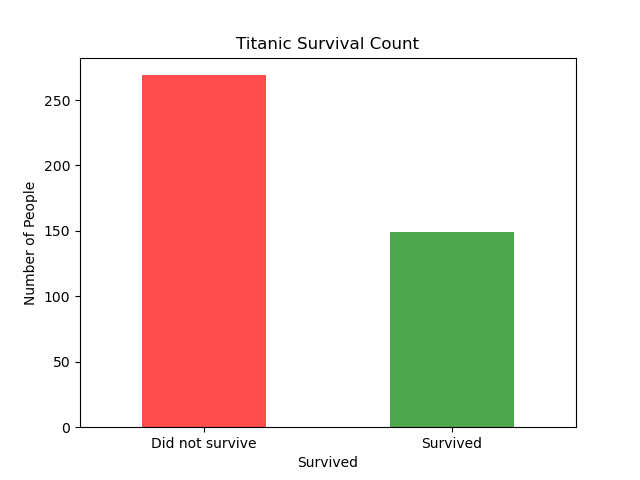
\includegraphics[scale=0.54]{./barchart2}
Looking at the percentages of males and females who survived in our test data. There were a total of 152 female passengers and 266 male passengers in the experiment. Going off of our percentages of 74.2\% of female passengers surviving and 18.8\% of males surviving, this will leave us with 113 female passengers and 50 male passengers that survived the Titanic within our test data. Combining both the training data with the test data there are a total of 466 female passengers and 843 male passengers. Using our previous values there would be about 346 female survivors and 159 male survivors. This leaves us with 120 female passengers and 684 male passengers that did not survive according to the combination of the testing and training data.
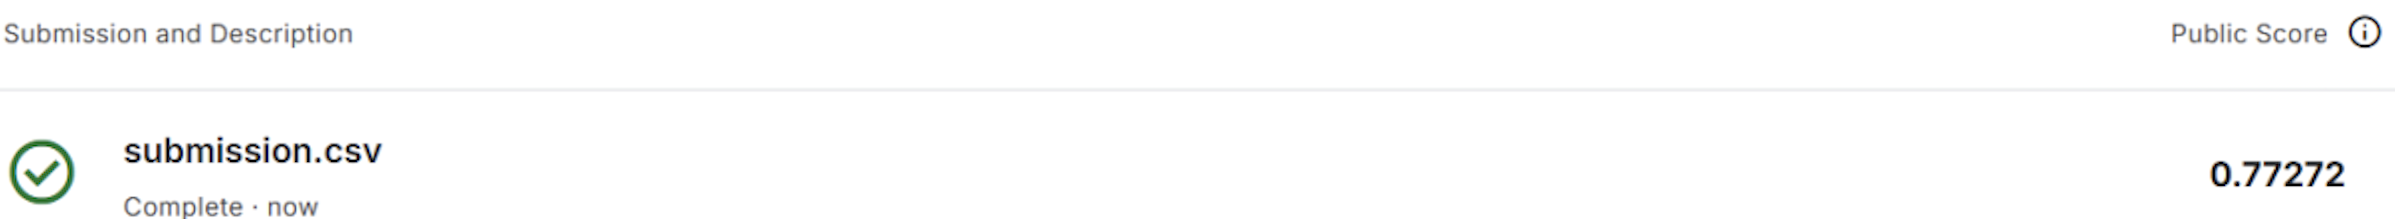
\includegraphics[scale=0.215]{./results.png}
\subsection{Analysis}

To start off the analysis of the data, looking at the cost per iterations of testing the data, we can see a clear decline in cost as iterations go on. The first iterations show costs of 0.693, 0.743, 0.730, and 0.719. These are noticeable declines for only being across 300 iterations of the data. Skipping to around 5000 iterations we see a cost of 0.488 showing us that across a larger number of iterations the cost is still declining. Going all the way to the end of the 9900 iterations we see 0.467. Comparing the declines from iterations 0-300 and the iterations from 5000-9900 we can see that over time the decline slows down by a large margin. Running more than 10000 iterations would help to see lower cost. However, the drop in cost would be so small that it is negligible and not necessary to do. The larger drops in cost show that the model is learning at a fast rate. The drops in cost become smaller as the iterations continue to go on, this shows us the model is converging on its lowest learning cost. This means that additional iterations will show very little improvement in learning cost for the model.

\section{Conclusion and Future Work}

\subsection{Conclusion}
In conclusion, our findings from running the logistic regression algorithm in our code showed that only a number of people were able to survive compared to the large number of people who did not. More specifically, our team has found that the majority of those who survived were predominately female, with only a small percentage of males surviving. To give more detail, that is equivalent to 113 females and 50 males surviving the Titanic disaster.  This data was quite intriguing because of the large gap between the number of female vs. male survivors. Also, to corroborate our findings, since this was a Kaggle competition to begin with, our team was able to submit the results of our code into the competition to test the accuracy of our solution/findings. As explained earlier in this report, our results were around 70\% accurate, which shows that our code effectively finds a solution for the Titanic Disaster problem.

Something else our team has discovered while implementing a solution for this problem is that, when there is a high number of iterations, the accuracy of the data tends to fall, which is shown in one of the graphs above. From this, our team has concluded that it is best to run this algorithm for predicting who will survive the Titanic with a number of iterations around 100 because, during this number of iterations, our algorithm tends to achieve the highest accuracy.
\subsection{Future Work}
For future directions of what our team could perhaps do to our algorithm, we had concluded that we need to find some solution or make some addition to our code that makes it so the logistic regression algorithm produces more accurate results. In order to check for this in the future, our team will continue submitting to the Kaggle competition webpage to ensure that the accuracy of our algorithm increases. This will make it so that our team will always try to improve the effectiveness of our algorithm. Our plan is to keep improving the code until the algorithm produces fully accurate results of who survived the Titanic.

On the other hand, our team will also try to use the concepts behind logistic regression learned from Assignment 1 in this course for future projects that may require. As such, our team will utilize what we learned doing this project to find solutions for far more difficult projects. In order to do so, our team must keep learning new strategies and new ways to improve our code so that it produces 100\% accurate results so that we can be sure that our understanding and implementation of logistic algorithms is adequate enough to find solutions for other problems.




\section{Contributions}

\subsection{Maeki Kashana}
\LIST{
\item Significant Contributions to the Final Report
    \LIST { \item Introduced the Research Problem
            \item Discussed, at length, any past work in the course that relates to this project
            \item Summarized findings and suggested possible future directions}
\item Created the README file
}
\subsection{Miguel Melo Ochoa}
\LIST{
\item Significant Contributions to the Code \& Model Submission
    \LIST { \item Introduced Kaggle Titanic ML Choice
            \item Implemented Logistic Regression for Kaggle Titanic ML Data
            \item Wrote Training, Testing, and Visualizing for the Logistic Regression Model}
\item Provided Supporting Result Images for group
}
\subsection{Alex Hayet}
\LIST{
\item
}
\subsection{Francisco Gomez}
\LIST{
\item Methodology and Technical Details
\item Provided ideas on how to implement the code
}

\REF {
\bibitem{titanic} Cubierski. W., ``Titanic - Machine Learning From Disaster,'' Kaggle.com, 2012.
}
\end{document}
